\chapter{Classical Mechanics}
\label{ch: classical-mechanics}
\section{Point Mass}
\subsection{Inclined plane I}
\label{prob: inclined_plane_pm_I}
\begin{figure}
    %Inclined Plane, horizontal plane
    \begin{center}
        \begin{tikzpicture}[thick]

            \def\ang{150}

            % Inclined plane
            \draw (0,0) coordinate[pos=1.,label={[above=1mm]{B}}] (B)  -- ++ (\ang:5) coordinate[label=above left:A] (A) |- (B) coordinate[pos=0.5] (O);


            % Angle Theta on the background wrt the inclined plane
            \begin{scope}[on background layer]
                \pic [draw, thick, -, "$\theta$", angle eccentricity=1.35, fill=gray!30, angle radius=10mm] {angle=A--B--O};
            \end{scope}

            % Horizontal plane
            \draw   (B) -- node[below=2mm] {$\mu$} ++ (3,0) coordinate[label=right:C] (aux);
            \path   [pattern={Lines[angle=45,distance={2pt},
                  line width=0.1pt]},
                  pattern color=gray]  (B) rectangle ++ (3,-0.2);
            
        
            % h
            \draw (O) -- node[midway,left=2mm] {$h$} (A);


            % Mass
            \begin{scope}[on background layer]
                \node (M) [draw=black,
                fill=yellow!60,
                minimum width=0.5cm,
                minimum height=0.5cm,
                anchor=north east,
                rotate=\ang,
                label=south west:$m$] at (A) {};
            \end{scope}

            % Speed in A, v_A
            \draw[thick, -{Triangle[]}] (M.center) -- ++ (\ang:-1) node[above right] {$\vec{v}_A$};

 
        \end{tikzpicture}
    \end{center}
    \caption{Setting of problem \ref{prob: inclined_plane_pm_I}.}
    \label{fig: inclined_plane_pm_I}
\end{figure}
A point mass $m$ is at the top of a plane inclined by an angle $\theta$ and of height $h$. At the end of such plane there is a rough horizontal plane which has a friction of with the point mass of coefficient $\mu$. At time $t=0$ the point mass is pushed with a speed $v_A$ parallel to the inclined plane. Determine:
\begin{enumerate}[(a)]
    \item The distance travelled on the horizontal plane by the point mass before stopping;
    \item the total time of motion.
\end{enumerate}
\begin{description}
    \item[Solution 1] We can first approach this problem from a dynamic--kinematic standpoint. This means that we: i) identify all the forces acting on the point mass; ii) use Newton's second law $\mb{F} = m \mb{a}$ to determine the acceleration and thus the motion, and iii) through the equations of motion we find the quantities we need. There are only two forces acting on the point: the constraint $\mb{N}$ directed perpendicularly to the inclined plane and pointing upwards, and the weight $\mb{P}$ directed vertically downwards (\cref{fig: free_body_diagram_pm_I}). 
    \begin{figure}
        \begin{center}
            \begin{tikzpicture}[
                force/.style={draw=black,fill=black},
                axis/.style={densely dashed,gray!50,font=\small},
                M/.style={rectangle,draw,fill=yellow!60,minimum width=0.5cm,minimum height=0.5cm,},
                m/.style={rectangle,draw=black,fill=lightgray,minimum size=0.3cm,thin},
                plane/.style={draw=black,fill=blue!10},
                string/.style={draw=red, thick},
                pulley/.style={thick},
            ]
                
                \def\ang{150}
                \def\down{-90}
                \def\arcr{0.5cm}
                \def\mg{1.8}
                \def\laxis{2.5}
                %\coordinate(X) at ({\mg*sin(\ang)},0);
                %\coordinate(Y) at (0,{\mg*cos(\ang)});

                %% Free body diagram of M
                \begin{scope}[rotate=\ang-180]
                    
                    \coordinate(M) at (0,0);

                    % Mass m
                    \node[M,transform shape] (M) {};
                    
                    
                    % Draw axes and help lines
                    \draw[thin,gray=!50, -{Triangle[]}] (M.center) -- (0,\laxis) node[right] {$+y$};
                    \draw[thin,gray=!50, -{Triangle[]}] (M.center) -- ++ (\laxis,0) node[right] {$+x$};
                    \draw[thin,gray=!50,dashed] (M.center) -- ++ (0,-\laxis) node[below left] {$-y$};
                    % Indicate angle. The code is a bit awkward.

                    %\draw[solid,shorten >=0.5pt] (\down-\ang:\arcr)
                    %    arc(\down-\ang:\down:\arcr);
                    %\node at (\down-0.5*\ang:1.3*\arcr) {$\alpha$};

                    % Forces
                    % Assuming that mg = \mg. The normal force will therefore be \mg*cos(alpha)
                    \draw[thick, -{Triangle[]}] (M.center) -- ++(0,-{\mg*cos(\ang)}) node[right=1mm] {$\vec{N}$};
                    % P components
                    \draw[thick, -, red] (M.center) -- ++ ({\mg*sin(\ang)},0)  node[above right=0.3mm, red] {$mg \sin \theta$};
                    \draw[thick, -, blue] (M.center) -- ++ (0,{\mg*cos(\ang)},0)  node[left=0.3mm, blue] {$mg \cos \theta$};
                    %\draw (M.west) -- ++(-1,0) node[left] {$f_R$};
                    %\draw (M.east) -- ++(1,0) node[above] {$T$};


                \end{scope}
                % Draw P. The code is put outside the rotated
                % scope for simplicity. No need to do any angle calculations. 
                \coordinate(P) at (0,-\mg);
                \draw[thick, -{Triangle[]}] (M.center) -- ++ (P) node[below] {$m\vec{g}$};
                
                \draw[thin,blue=!50,dashed,rotate=\ang] (P) -- ++ ({\mg*sin(\ang)},0);
                \draw[thin,red=!50,dashed,rotate=\ang] (P) -- ++ (0,{\mg*cos(\ang)});


            \end{tikzpicture}
        \end{center}
        \caption{Free--body diagram for problem \ref{prob: inclined_plane_pm_I}.}
        \label{fig: free_body_diagram_pm_I}
    \end{figure}
    Let us separate the problem in two parts: the motion on the inclined plane from $A$ to $B$ and the motion on the horizontal plane from $B$ to $C$. In $AB$, let us put the $x$ axis and the $y$ axis along the inclined plane and perpendicularly to it, respectively (\cref{fig: free_body_diagram_pm_I}). Newton's law then becomes
    \begin{align}
        x: \, & P_x = m a \label{eq: acc_inclined_plane_pm_I} \\
        y: \, & N - P_y = 0,
    \end{align} 
    where the acceleration along $y$ is zero as the point only slides along the plane and not perpendicularly to it. How do we find the components of the weight? We argue that the angle between $\mb{P}$ and the negative $y$ axis is the inclination angle $\theta$: this can be seen immediately if ones realizes that the $y$ axis and $\mb{P}$ are orthogonal to the inclined plane and its base, respectively, so that the angle between these two pairs of sides have to be equal (\cref{fig: angle_P_inclined_plane}). Then
    \begin{gather}
        P_x = P \sin \theta = mg \sin \theta \label{eq: P_x_inclined_plane_pm_I} \\
        P_y = P \cos \theta = mg \cos \theta.
    \end{gather}
    Then, replacing $P_x$ from \cref{eq: P_x_inclined_plane_pm_I} into \cref{eq: acc_inclined_plane_pm_I} we get an expression for the acceleration in the tract $AB$
    \begin{equation}
        mg \sin \theta = ma_{AB} \Rightarrow a_{AB} = g \sin \theta.
    \end{equation} 
    The point acceleration is constant, thus the motion will be uniformly accelerated. The laws of motion are the following
    \begin{align}
        x(t) & = x_0 + v_0 t + \frac{1}{2} a t^2 \label{eq: x_uam} \\
        v(t) & = v_0 + at \label{eq: v_uam},
    \end{align}
    where $x_0$ and $v_0$ are the initial position and speed of the point, respectively, $a$ is the (constant) acceleration and $t$ is time.,
    What we need to find is the speed that the point has in $B$, $v_B$, as this will be the initial speed for the successive motion along the horizontal plane. We can find this quantity using the time--less formula for the uniformly accelerated motion\footnote{This formula is simply obtained by eliminating $t$ from \cref{eq: x_uam,eq: v_uam}.}
    \begin{equation}
        \label{eq: timeless_formula_uam}
        v_f^2 = v_i^2 + 2 a \Delta x,
    \end{equation}
    where $\Delta x$ is the space travelled between the initial and final time, and $a$ is constant. In our case $\Delta x = h/ \sin \theta$ is the length of the inclined plane, so that we have
    \begin{equation}
        \label{eq: speed_inclined_plane_pm_I}
        v_B = \sqrt{v_A^2 + 2 g h}.
    \end{equation}
    Now let us study the second part of the problem, that is the motion on the horizontal plane. In $BC$ the point is subject to three forces: $\mb{P}$ and $\mb{N}$ on the $y$ axis which balance themselves, and the friction $\mb{f}_a = -\mu N \hat{v}$, directed to the left along the $x$ axis. We can write
    \begin{align}
        x: \, & - \mu mg = m a_{BC} \\
        y: \, & N - P = 0,
    \end{align}
    where we have used that $N=P$ on the horizontal plane. Again the acceleration is constant in this tract
    \begin{equation}
        a_{BC} = - \mu g,
    \end{equation}
    so that we can calculate the distance inverting \cref{eq: timeless_formula_uam} for the distance travelled $\Delta x = d$
    \begin{gather}
        v_C^2 = v_B^2 + 2 a_{BC} d \Rightarrow \notag \\
        d = \frac{v_B^2}{2 \mu g} = \mybox{\frac{v_A^2}{2 \mu g} + \frac{h} {\mu}} \label{eq: d_inclined_plane_pm_I},
    \end{gather}
    where we have used that $v_C = 0$, because the problem asks for the distance travelled until the point stops, and we have taken $v_B$ from \cref{eq: speed_inclined_plane_pm_I}. Eq. \eqref{eq: d_inclined_plane_pm_I} gives us the distance travelled on the horizontal plane: if we want the \emph{total} distance we will need to add the length of the inclined plane $L = h/\sin\theta$. As for the total time of motion, we have again to add the time of the two parts, $AB$ and $BC$. 
    QED
    \item[Solution 2] Another way to go at this problem is using the formalism of mechanical energy. Specifically, we can use the law of mechanical energy conservation whenever only conservative forces are at play, and the theorem of kinetic energy where there is dissipation.

\end{description}
%%%%%%%%%%%%%%%%%%%%%%%%%%%%%%%%%%%%%%%%%%%%%%%%%%%
%%%%%%%%%%%%%%%%%%%%%%%%%%%%%%%%%%%%%%%%%%%%%%%%%%%
%%%%%%%%%%%%%%%%%%%%%%%%%%%%%%%%%%%%%%%%%%%%%%%%%%%
%%%%%%%%%%%%%%%%%%%%%%%%%%%%%%%%%%%%%%%%%%%%%%%%%%%
\section{Solid Bodies}
\subsection{Circular track and spring I}
\label{prob: circ_track_spring}
\begin{figure}
    % Circular track
    \begin{center}
        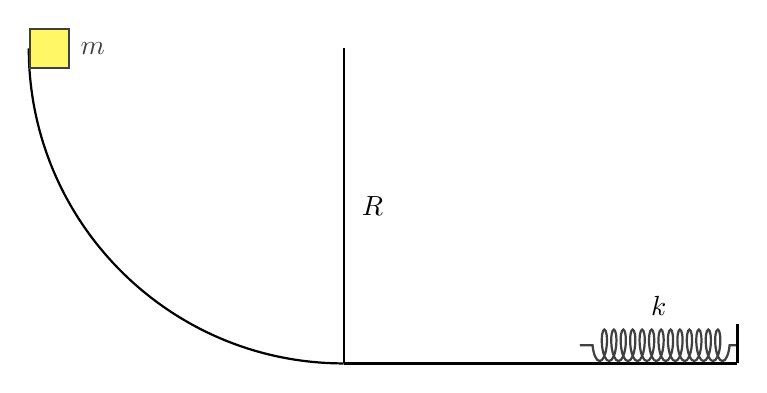
\begin{tikzpicture}[black!75,thick]
 
            % Coordinates
            \coordinate(A) at (0,0);
            \coordinate(B) at (0,4);
            \coordinate(C) at (4,4);
            \coordinate(D) at (4,0);
            \coordinate(E) at (9,0);
            \coordinate(F) at (9,0.23);
            \coordinate(G) at (7,0.23);
        
        
            % Arc
            \draw[black,thick] (B) arc[start angle=180, end angle=270, radius=4];
            \draw[black,thick] (D) -- (E);
            \draw[black,thick] (C) -- (D) node[midway,right=0.1cm,black]{$R$}; 
        
        
            % Mass
            \node[draw,
                fill=yellow!60,
                minimum width=0.5cm,
                minimum height=0.5cm,
                anchor=west,
                label=east:$m$] at (B) {};
        
        
            % Spring 
            \draw
            [
                decoration={
                    coil,
                    aspect=0.3, 
                    segment length=1.2mm, 
                    amplitude=2mm, 
                    pre length=1mm,
                    post length=1mm},
                decorate
            ] (F) -- (G) 
                node[midway,above=0.25cm,black]{$k$}; 
            \draw[black,thick] (9, 0) -- (9, 0.5);
             
        \end{tikzpicture}
    \end{center}
    \caption{Setting of problem \ref{prob: circ_track_spring}.}
    \label{fig: circular_track1}
\end{figure}

A body of mass $m$ is at the top of a circular track of radius $R$, and is left to fall at time $t=0$ with zero initial speed. At the end of the track there's a horizontal plane with a spring of stiffness $k$ at the end (\cref{fig: circular_track1}).
Determine:
\begin{enumerate}[(a)]
    \item the speed of the body when the spring is compressed by $\Delta x$, and the variation in potential energy at that point;
    \item assuming that the surface is rough and the work of the friction is $W_f < 0$, determine the maximum compression of the spring.
\end{enumerate}
\begin{description}
    \item[Solution]
    \begin{enumerate}[(a)]
        \item In the first part of the problem there is no friction and all the forces at play (gravitational and elastic) are conservative, hence we can use the conservation of mechanical energy to study the body's dynamics. Let us call $U^g = mgh$ and $U^e=\frac{1}{2}k\Delta x^2$ the gravitational and elastic potential energy, respectively. We have
        \begin{gather}
            E_i = E_f \Leftrightarrow K_i + U^g_i + U^e_i = K_f + U^g_f + U^e_f \Leftrightarrow \notag \\
            mgR = \frac{1}{2}mv_f^2 + \frac{1}{2}k\Delta x^2, \label{eq: energy_conservation1}
        \end{gather}
        where $i$ and $f$ correspond to $t=0$ and the time when the spring is compressed by $\Delta x$, respectively. $K_i=0$ since $v_i=0$, $U_i^e=0$ because the spring is not compressed at $t=0$, and $U_f^g=0$ since the height is zero on the horizontal plane. Solving \cref{eq: energy_conservation1} for $v_f$ we have
        \begin{gather}
            \frac{1}{2} m v_f^2 = mgR - \frac{1}{2}k \Delta x^2 \Rightarrow \notag \\
            \mybox{v_f = \sqrt{2gR - \frac{k}{m}\Delta x^2}}.
        \end{gather}
        QED
        \item The second part includes friction and thus a non--conservative force. As a consequence mechanical energy is not conserved, and we need to use another equation to study our problem. Specifically, we will use the kinetic energy theorem
        \begin{equation}
            \label{eq: kin_energy_th}
            W_{tot} = \Delta K,
        \end{equation}
        where $W_{tot}$ is the work generated by \emph{all} the forces acting upon the body in a given time interval $\Delta t$, and $ \Delta K $ is the variation in kinetic energy during $\Delta t$. In our case, the two time points are $t=0$, and the instant when the spring is maximally compressed which we'll call $t_m$. We then have, for the lhs and rhs
        \begin{gather*}
            W_{tot} = W_g + W_e + W_f = mgR - \frac{1}{2}k \Delta x_{max}^2 + W_f \\
            \Delta K = 0,
        \end{gather*}
        where we have used that $ W = -\Delta U $ for a conservative force. Notice that $\Delta K = 0$, because the body starts off with zero speed, and at $t_m$ the spring is maximally compressed, which also means the body has zero speed. Putting it all together we get
        \begin{equation}
            mgR - \frac{1}{2}k \Delta x_{max}^2 + W_f = 0,
        \end{equation}
        which, solving for $\Delta x$, becomes
        \begin{gather}
            \frac{1}{2}k \Delta x^2 = mgR + W_f \Rightarrow \notag \\
            \mybox{\Delta x = \sqrt{\frac{2}{k} \Bigl( mgR + W_f \Bigr)}}.
        \end{gather}
        QED
    \end{enumerate}  
\end{description}
%%%%%%%%%%%%%%%%%%%%%%%%%%%%%%%%%%%%%%%%%%%%%%%%%%%
%%%%%%%%%%%%%%%%%%%%%%%%%%%%%%%%%%%%%%%%%%%%%%%%%%%
%%%%%%%%%%%%%%%%%%%%%%%%%%%%%%%%%%%%%%%%%%%%%%%%%%%
%%%%%%%%%%%%%%%%%%%%%%%%%%%%%%%%%%%%%%%%%%%%%%%%%%%
\subsection{Inclined plane I}
\label{prob: inclined_plane_I}
A solid body of mass $m_1$ and radius $R$ is on a plane inclined by angle $\theta$. At the upper end of the solid body is attached an ideal rope, which supports a mass $m_2$. The system is initially still, the rope is tight, and the pulley is ideal. At time $t=0$, the mass $m_2$ is left free to move, and it starts to fall downward, causing the sphere to climb up the plane. The solid body's motion is of pure rolling. Determine:
\begin{enumerate}[(a)]
    \item the acceleration of mass $m_2$ and the tension of the rope $T$;
    \item the speed of the mass $m_2$ after falling by $h$.
\end{enumerate}

\begin{figure}
    \begin{center}
        \def\iangle{35} % Angle of the inclined plane
        \def\down{-90}
        \def\arcr{0.5cm} % Radius of the arc used to indicate angles
        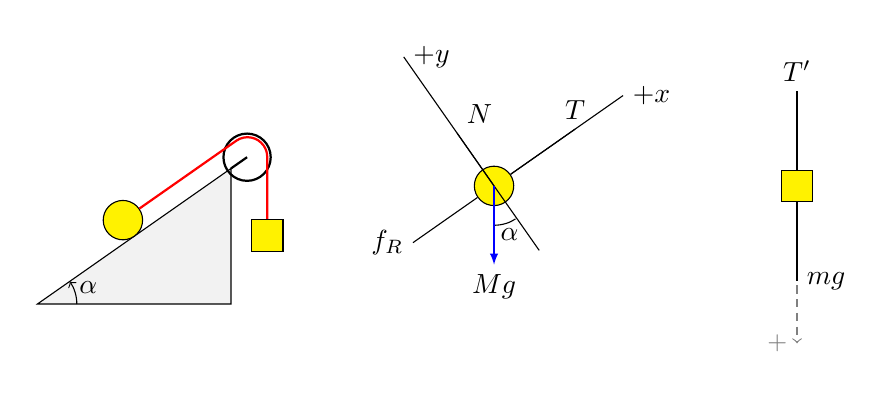
\begin{tikzpicture}[
            force/.style={>=latex,draw=blue,fill=blue},
            axis/.style={densely dashed,gray,font=\small},
            M/.style={circle,draw,fill=yellow,minimum size=0.5cm,thin},
            m/.style={rectangle,draw=black,fill=yellow,minimum size=0.4cm,thin},
            plane/.style={draw=black,fill=gray!10},
            string/.style={draw=red, thick},
            pulley/.style={thick},
        ]
    
            
        \matrix[column sep=1cm] {
            %% Sketch
            \draw[plane] (0,-1.5) coordinate (base)
                            -- coordinate[pos=0.5] (mid) ++(\iangle:3) coordinate (top)
                            |- (base) -- cycle;
            \path (mid) node[M,rotate=\iangle,yshift=0.25cm] (M) {};
            \draw[pulley] (top) -- ++(\iangle:0.25) circle (0.3cm)
                        ++ (90-\iangle:0.5) coordinate (pulley);
            \draw[string] (M.east) -- ++(\iangle:1.5cm) arc (90+\iangle:0:0.25)
                        -- ++(0,-1) node[m] {};
    
            \draw[->] (base)++(\arcr,0) arc (0:\iangle:\arcr);
            \path (base)++(\iangle*0.5:\arcr+5pt) node {$\alpha$};
            %%
    
        &
            %% Free body diagram of M
            \begin{scope}[rotate=\iangle]
                \node[M,transform shape] (M) {};
                % Draw axes and help lines
    
                {[axis,->]
                    \draw (0,-1) -- (0,2) node[right] {$+y$};
                    \draw (M) -- ++(2,0) node[right] {$+x$};
                    % Indicate angle. The code is a bit awkward.
    
                    \draw[solid,shorten >=0.5pt] (\down-\iangle:\arcr)
                        arc(\down-\iangle:\down:\arcr);
                    \node at (\down-0.5*\iangle:1.3*\arcr) {$\alpha$};
                }
    
                % Forces
                {[force,->]
                    % Assuming that Mg = 1. The normal force will therefore be cos(alpha)
                    \draw (M.center) -- ++(0,{cos(\iangle)}) node[above right] {$N$};
                    \draw (M.west) -- ++(-1,0) node[left] {$f_R$};
                    \draw (M.east) -- ++(1,0) node[above] {$T$};
                }
    
            \end{scope}
            % Draw gravity force. The code is put outside the rotated
            % scope for simplicity. No need to do any angle calculations. 
            \draw[force,->] (M.center) -- ++(0,-1) node[below] {$Mg$};
            %%
    
        &
            %%%
            % Free body diagram of m
            \node[m] (m) {};
            \draw[axis,->] (m) -- ++(0,-2) node[left] {$+$};
            {[force,->]
                \draw (m.north) -- ++(0,1) node[above] {$T'$};
                \draw (m.south) -- ++(0,-1) node[right] {$mg$};
            }
    
        \\
        };
        \end{tikzpicture}
    \end{center}
    \caption{Setting of the problem \ref{prob: inclined_plane_I}.}
    \label{fig: inclined_plane}
\end{figure}

\begin{description}
    \item[Solution 1] 
    \begin{enumerate}[(a)]
        \item We will study the dynamics of the above system considering the cardinal equations 
        \begin{gather}
            \mb{F}_2 = m_2 \mb{a}_2 \\
            \mb{F}^{ext} = m_2 \mb{a}_{CM} \\
            \mb{M} = I_o \bm{\alpha}.
        \end{gather}  
        We then have to fix a coordinate system for each of the two bodies and find the components of the forces and the torques. Let us consider the two free--body diagrams as in \cref{fig: inclined_plane}. First let us specify what are the forces acting on the two bodies. On $m_1$ we have
        \begin{itemize}
            \item $\mb{P}_1$ acting on the center of mass downward;
            \item $\mb{T}$ acting on the upper edge towards the positive $x$--axis;
            \item $\mb{N}$ acting on the contact pointing towards the positive $y$--axis;
            \item $\mb{f}$ the friction acting on the contact point and directed along the $x$--axis -- notice that, since we are dealing with static friction, we do not know a priori what its verse is: it could be either the positive or the negative $x$--axis, and we can find this out only by solving the cardinal equations. For now we assume that $\mb{f}$ is along the negative $x$--axis.
        \end{itemize}
        On $m_2$ on the other hand we have 
        \begin{itemize}
            \item $\mb{P}_2$ directed downward;
            \item $\mb{T}$ directed upward.
        \end{itemize}
        Then for $m_2$ we can immediately write
        \begin{equation}
            P_2 - T = m_2 a_2.
        \end{equation}
        As for $m_1$, we have, along the $x$--axis
        \begin{equation}
            T - P_1 \sin \theta - f = m_1 a_{CM}.
        \end{equation}
        As for the momentum equation, let us consider the contact point as the reference to calculate all our quantities. Then $\mb{P}_1$ will have an arm equal to $R$; $\mb{T}$ has an arm $2R$, whereas $\mb{N}$ and $\mb{f}$ have zero arm and thus zero torque. Let us remember that the torque is defined as
        \begin{equation}
            \mb{M}_o = \mb{r}_o \times \mb{F},    
        \end{equation} 
        where $o$ is the reference point, and $\mb{r}$ is the arm of the force $\mb{F}$ from point $o$. Now we can immediately say that the tension $\mb{T}$ has a torque directed inwards with module $M_T = 2RT$, whereas the weight $\mb{P}_1$ has a torque directed outwards with module $P_1 R \sin (\pi - \theta)$.
        We then have
        \begin{equation}
            2RT - P_1 R \sin(\pi - \theta) = I_c \alpha,
        \end{equation}
        where $I_c$ is the moment of inertia of the solid body evaluated with respect to the contact point $C$, which we can find using the Huygens--Steiner theorem\footnote{Also called the \emph{parallel axis theorem}.}:
        \begin{equation}
            \label{eq: Ic_rolling}
            I_c = I_{CM} + m_1 R^2 = B m_1 R^2 + m_1 R^2 = (B+1) m_1 R^2 = \mathcal{B} m_1 R^2.
        \end{equation}
        In \cref{eq: Ic_rolling} we have used the fact that $I_{CM} = B m_1 R^2$, where $B$ will depend on the specific shape of the solid body. For instance, $B=1/2$ for a homogeneous cylinder, while $B=2/5$ for a homogeneous sphere. We have then called $\mathcal{B} = B+1$.
        So, putting all together we have
        \begin{equation}
            \label{eq: system_1}
            \begin{cases}
            m_1: 
            \begin{cases}
                T - P_1 \sin \theta - f = m_1 a_{CM} \\
                2RT - R P_1 \sin (\pi - \theta) = I_o \alpha
            \end{cases} \\
            m_2:
            \begin{cases}
                P_2 - T = m_2 a_2,
            \end{cases}
        \end{cases}
        \end{equation}
        which is a system of three equations with five unknowns: $T, f, a_{CM}, a, \alpha$. We then need two more equations to be able to solve the system, and we can resort to geometric relations between the accelerations. Indeed, the pure rolling of the sphere causes the point on the upper edge to have an acceleration twice as big as the center of mass'
        \begin{gather}
            a_2 = 2 a_{CM} \notag \\
            a_{CM} = \alpha R \Leftrightarrow \alpha = a_{CM}/R \notag \\
            a_{CM} = \frac{a_2}{2} \\
            \alpha = \frac{a_2}{2R}
        \end{gather}
        respectively, and these are the two further equations that we need to solve the system in \cref{eq: system_1}:
        \begin{equation}
            \label{eq: system_2}
            \begin{cases}
                T - P_1 \sin \theta - f = m_1 \frac{a_2}{2} \\
                2RT - P_1R \sin(\pi - \theta) = I_c \frac{a_2}{2R} \\
                P_2 - T = m_2 a_2.
            \end{cases}
        \end{equation}
        We can find $a_2$ by isolating $T$ from the third equation and substituting its expression in the first, to find
        \begin{equation}
            \label{eq: a_2_inclined_plane_rolling}
            a_2 = \frac{2P_2 - P_1 \sin(\pi - \theta)}{2 m_2 R + I_c/(2R)} R = \mybox{2 \frac{2m_2 - m_1 \sin\theta}{4m_2 + \mathcal{B} m_1} g}
        \end{equation}
        where we have exploited the fact that $\sin (\pi - \theta) = \sin \theta$.
        As for the tension, we can now use the third equation from the system in \cref{eq: system_2} with the expression for $a_2$ in \cref{eq: a_2_inclined_plane_rolling} to find
        \begin{gather}
            T = P_2 - m_2 a_2 = m_2 g \biggl( 1- 2 \frac{2m_2 - m_1 \sin\theta}{4m_2 + \mathcal{B} m_1} g \biggr) \notag \\
            = \mybox{\frac{m_1 m_2}{4m_2 + \mathcal{B} m_1} \Bigl( \mathcal{B} + 2 \sin \theta \Bigr) g} \label{eq: tension_inclined_plane_rolling}.
        \end{gather}
        In \cref{eq: a_2_inclined_plane_rolling,eq: tension_inclined_plane_rolling}, we can replace $\mathcal{B}$ with the corresponding values for a homogeneous cylinder or a sphere, to obtain the expressions for these two solid bodies.
        ***** insert table with values of $B$ and $\mathcal{B}$ for cylinder and sphere *******.
        QED
        \item The speed of...
    \end{enumerate}

    \item[Solution 2 - point (a) with matrices] An interesting way to solve....
\end{description}